% THIS IS SIGPROC-SP.TEX - VERSION 3.1
% WORKS WITH V3.2SP OF ACM_PROC_ARTICLE-SP.CLS
% APRIL 2009
%
% It is an example file showing how to use the 'acm_proc_article-sp.cls' V3.2SP
% LaTeX2e document class file for Conference Proceedings submissions.
% ----------------------------------------------------------------------------------------------------------------
% This .tex file (and associated .cls V3.2SP) *DOES NOT* produce:
%       1) The Permission Statement
%       2) The Conference (location) Info information
%       3) The Copyright Line with ACM data
%       4) Page numbering
% ---------------------------------------------------------------------------------------------------------------
% It is an example which *does* use the .bib file (from which the .bbl file
% is produced).
% REMEMBER HOWEVER: After having produced the .bbl file,
% and prior to final submission,
% you need to 'insert'  your .bbl file into your source .tex file so as to provide
% ONE 'self-contained' source file.
%
% Questions regarding SIGS should be sent to
% Adrienne Griscti ---> griscti@acm.org
%
% Questions/suggestions regarding the guidelines, .tex and .cls files, etc. to
% Gerald Murray ---> murray@hq.acm.org
%
% For tracking purposes - this is V3.1SP - APRIL 2009

\documentclass{sig-alternate}
\setlength{\paperheight}{11in}
\setlength{\paperwidth}{8.5in}
\usepackage[pass]{geometry}
\usepackage{verbatim}
\usepackage{url}
\usepackage{listings}
\usepackage{color}
\usepackage{multicol}
\usepackage{paralist}
\usepackage{comment}
\usepackage{hyperref}

\newcommand{\figref}[1]{Figure~\ref{#1}}
\newcommand{\tableref}[1]{Table~\ref{#1}}
\newcommand{\secref}[1]{Section~\ref{#1}}

\definecolor{dkgreen}{rgb}{0,0.6,0}
\definecolor{gray}{rgb}{0.5,0.5,0.5}
\definecolor{mauve}{rgb}{0.58,0,0.82}

\lstset{frame=tb,
  language=Java,
  aboveskip=3mm,
  belowskip=3mm,
  showstringspaces=false,
  columns=flexible,
  basicstyle={\small\ttfamily},
  numbers=none,
  numberstyle=\tiny\color{gray},
  keywordstyle=\color{blue},
  commentstyle=\color{dkgreen},
  stringstyle=\color{mauve},
  breaklines=true,
  breakatwhitespace=true
  tabsize=3
}

\begin{document}

\title{JPF Verification of Habanero Java Programs using Gradual Type Permission Regions\titlenote{Research funded by NSF grant CCF-1302524}}

%
% You need the command \numberofauthors to handle the 'placement
% and alignment' of the authors beneath the title.
%
% For aesthetic reasons, we recommend 'three authors at a time'
% i.e. three 'name/affiliation blocks' be placed beneath the title.
%
% NOTE: You are NOT restricted in how many 'rows' of
% "name/affiliations" may appear. We just ask that you restrict
% the number of 'columns' to three.
%
% Because of the available 'opening page real-estate'
% we ask you to refrain from putting more than six authors
% (two rows with three columns) beneath the article title.
% More than six makes the first-page appear very cluttered indeed.
%
% Use the \alignauthor commands to handle the names
% and affiliations for an 'aesthetic maximum' of six authors.
% Add names, affiliations, addresses for
% the seventh etc. author(s) as the argument for the
% \additionalauthors command.
% These 'additional authors' will be output/set for you
% without further effort on your part as the last section in
% the body of your article BEFORE References or any Appendices.

\numberofauthors{4} %  in this sample file, there are a *total*
% of EIGHT authors. SIX appear on the 'first-page' (for formatting
% reasons) and the remaining two appear in the \additionalauthors section.
%
\author{
\alignauthor
Peter Anderson\\
       \affaddr{Brigham Young University}\\
       \affaddr{Provo, Utah}\\
       \email{anderson.peter@byu.edu}
\alignauthor
Nick Vrvilo\\
    \affaddr{Rice University}\\
    \affaddr{Houston, Texas}\\
    \email{nv4@rice.edu}
\and
\alignauthor
Eric Mercer \\
       \affaddr{Brigham Young University}\\
       \affaddr{Provo, Utah}\\
       \email{egm@cs.byu.edu}
\alignauthor
Vivek Sarkar \\
        \affaddr{Rice University}\\
        \affaddr{Houston, Texas}\\
        \email{vsarkar@rice.edu}
}

    
% There's nothing stopping you putting the seventh, eighth, etc.
% author on the opening page (as the 'third row') but we ask,
% for aesthetic reasons that you place these 'additional authors'
% in the \additional authors block, viz.
\additionalauthors{Additional authors: John Smith (The Th{\o}rv{\"a}ld Group,
email: {\texttt{jsmith@affiliation.org}}) and Julius P.~Kumquat
(The Kumquat Consortium, email: {\texttt{jpkumquat@consortium.net}}).}
\date{30 July 1999}
% Just remember to make sure that the TOTAL number of authors
% is the number that will appear on the first page PLUS the
% number that will appear in the \additionalauthors section.

\maketitle
\begin{abstract}
The Habanero Java Library (HJ-lib) is a Java 8 library implementation of the
Habanero Java (HJ) programming model. Calls into this pure Java library provide
support for all HJ primitives, including async, finish, and phasers. In
previous work, we presented VR, a
custom verification runtime designed to be used within Java Pathfinder (JPF) to
verify a subset of HJ programs. In this work, we present VR-lib, a library
implementation of HJ, which supports verification of a larger subset of
programs than VR. Additionally, we present the implementation of gradually typed
permission regions (GPRs). PRs provide a building block for dynamically
detecting violations of conditions sufficient to guarantee race-freedom.
Lastly, we present results for benchmarks using PRs in combination with VR-lib
to verify HJ programs.  
\end{abstract}
%\category{D.2.4}{Software/Program Verification}{Model Checking}
%\terms{Model Checking}
%\keywords{Model checking, high performance computing, Java Pathfinder} % NOT required for Proceedings
%\section{Introduction}
Despite the explosion in multi-core hardware for general purpose
computing, writing programs to take advantage of the available
processing power is a task reserved for expert
developers. Parallel programming models are nuanced with non-trivial 
language semantics, and the first programs from the uninitiated have
more in common with sequential execution than parallel performance due
to excessive synchronization, or worse, those programs are
fraught with concurrency errors due to an absence of needed
synchronization. Parallel semantics is not the normal mental model for
most programmers, and as a result, parallelism is employed little,
deployed incorrectly, or exclusively reserved for the expert users
which are not found in abundance.

The Habanero extreme scale software research project intends to bring
multi-core programming to the masses by providing languages,
compilers, run-time systems, and tools to support programmers that are
not experts in concurrency. Habanero itself is a task-parallel
programming model built around lightweight asynchronous tasks and data
transfers. As such, rather than manipulating processes, threads, and
synchronization for concurrent execution, the programmer identifies
sections of the program that can run concurrently as tasks using
simple annotations in the sequential code. An implementation of
Habanero would then shoulder the complexity of the parallel execution
and absolve the programmer of that responsibility. The
programmer now focuses on the high-level task constructs while an
implementation worries about how to correctly implement and
synchronize those constructs.

Aside from the simplified task-parallel programming model, Habanero
gives some limited correctness guarantees. It defines safe subsets of
the language that preserve correctness in regards to concurrent
interactions. For example, programs that only create tasks and join
on their termination are free of deadlock, support serialization (i.e.,
removing all the annotations yields a sequential program that gives
the same computation), and in the absence of data-race (i.e.,
conflicting concurrent accesses to shared memory), those same programs
are deterministic. In a safe subset, a programmer does not need to
worry about concurrent interactions between tasks beyond data-race.

Habanero Java (\hj) is the most widely deployed implementation of the
Habanero model, and it has been adopted as a pedagogical language for
teaching concurrency \cite{Cave:2011:HNA:2093157.2093165}; however,
there is a gap between the theory of the language with its safe subsets
and the implementation in regards to test and validation.  When operating
within a safe subset of the language or outside for
performance, there is no easy way to determine when and if a program
is free of data-race---a necessary condition for determinism. Even
debugging computation is non-trivial as the \hj\ implementation is
complex, so a user has no obvious method to track a task, let alone
control its execution, using a conventional debugger. As a result,
inefficient code inspection, run-time failures, and
\emph{printf}-debugging are the primary techniques for test and validation.

This paper presents research to address debugging, test, and
validation for task parallel programming models such as Habanero. The
first contribution is a new implementation of Habanero for Java in the
form of a library (\hjv). The implementation trades performance for
simplicity and correctness. It does this by using Java threads for
each task, and using global locks with conditions for features of
Habanero that require mutual exclusion and complex synchronization. As
such, it is well suited for test and validation since a conventional
debugger is able to inspect and control the execution of tasks (e.g.,
Java threads). Additionally, weighing in with only 32
classes and around 1,300 lines of code, the library is an
order of magnitude less complex than even the most simple
implementations in the \hj\ distribution. Careful manual inspection of
the code base, which is conveniently small, with extensive testing and
verification, reasonably ensure a high degree of confidence in its correctness and supports the
claim that \hjv\ preserves all behaviors allowed by the Habanero
semantics. That said, finding deadlock and data-race in an input
program is still a difficult challenge as is enumerating behaviors for test in non-deterministic programs.

The \hjv\ library enables model checking for \hj\ programs. Model
checking exhaustively enumerates program behavior, and in the case of
task-parallel programming models, it reasons over task schedules to
prove the absence of errors. The Java Pathfinder model checker (\jpf)
is able to directly verify freedom from deadlock and data-race in
\hj\ programs using \hjv\ as the Habanero implementation because \hjv\ employs a one-to-one
mapping between tasks and threads. The verification leverages the
native support for threads and locks in \jpf\ to automatically explore all possible
ways to schedule concurrent tasks. Such an approach is not possible
using the other Habanero implementations in the \hj\ distribution
because \jpf\ does not know where to schedule. The model checking is effective for verifying the
\hjv\ implementation beyond manual inspection and proving small
programs correct, but it does not scale to larger programs.

The second contribution to debugging, test, and validation is an
implementation in \jpf\ of a sound algorithm for the validation of
task-parallel programming models such as Habanero that is able to
detect programs that are free of deadlock and data-race (\jpfhj). It also enumerates all outcomes that arise from non-determinism in sequencing isolated atomic blocks. The
algorithm still employs model checking with the \hjv\ library as
before; however, to scale to larger input programs, the algorithm uses
permission regions to annotate atomic blocks of read/write operations
on shared memory. These atomic blocks effectively reduce the number of
schedules that must be considered to prove a program correct.

Permission regions are program annotations that announce how a task
interacts with shared memory (i.e., reading or writing), and over what
region of code that interaction takes place
\cite{Westbrook:2011:PRR:2341616.2341627,
  Westbrook:2012:PPR:2367163.2367201}. During execution, auxiliary
data structures track access on those memory regions and signal an
error on any conflicting access. Permission regions have been shown
effective in dynamically detecting data-race at run-time.

\jpfhj\ includes an implementation of permission regions and a
specialized scheduling algorithm to reduce the number of explored
schedules needed to show a program free of deadlock and data-race. The
new algorithm only preempts at the entrance to permission regions and isolated atomic blocks to
schedule threads.  As stated previously, the new algorithm is sound,
meaning that it may reject programs that are actually correct if the
permission regions are too big, but effective at controlling state explosion. The
algorithm does report a witness to any discovered deadlock or
data-race violation which can be used to validate the error with the
debugger. If the error is a false report due to the size of the
regions, then the witness provides insight on how to reduce the size of
the permission regions. This new algorithm together with the
simplified run-time provide needed support for debug, test, and
validation of task parallel programs.

The principle contributions described in this paper are summarized as
\begin{compactitem}
\item \hjv: a verification specific implementation of Habanero for Java as a Java library that is extensively tested through model checking with \jpf\ and is amenable to conventional debugging;
\item \jpfhj: an implementation of permission regions in the \jpf\ model checker with a sound algorithm that only schedules on permission regions and isolated atomic blocks to prove a program free of deadlock and data-race; and 
\item an empirical study showing the impact of permission regions on the complexity of model checking over a set of benchmarks.
\end{compactitem}
The \hjv\ library and \jpfhj\ specialization are available for
download at: \url{http://javapathfinder.org/jpf-hj/}.

\section{Introduction}
The increasing use of multicore processors is motivating the use of parallel programming. However, it is very difficult to write concurrent programs that are free from bugs. When programs execute different instructions simultaneously, different thread schedules and memory access patterns are observed that give rise to various issues such as data-races, deadlocks etc. To make writing concurrent programs easier, Rice University developed Habanero Java Programming model \cite{Cave:2011:HNA:2093157.2093165}. It provides safety guarantees such as deadlock freedom, deterministic output and serialization for subsets of constructs provided in the programming model. These guarantees hold only in the absence of data-races. The Habanero Java library (HJ-Lib) \cite{hj-lib} is a Java 8 library implementation of the Habanero Java programming model.

VR-lib \cite{Anderson:2015:JVH:2693208.2693245}, a verification runtime for HJ programs was built at Brigham Young University. VR-lib facilitates the verification of HJ programs using JPF. VR-lib can be used along with JPF to build computation graphs of HJ programs. A Computation Graph (CG) is an acyclic directed graph that consists of a set of nodes, where each node represents a step consisting of some sequential execution of the program and a set of edges that represent the ordering of the steps. A CG stores the memory locations accessed and updated by each of the operators. It also correctly reflects the control flow structure of the program.

The CGRaceDetector listener presented in this work monitors the various object creations and destructions, instruction executions etc to build a computation graph for the HJ program under a single schedule. It later analyzes this graph to verify any data access violations to report data races. For structurally deterministic programs, verifying the HJ program under a single schedule is enough to detect data races.

Section 2 of this paper presents an overview of the Habanero Java programming model and gives a brief description for the various parallel constructs of HJ language. Section 3 describes the computation graphs and its various elements. It also gives the implementation details of computation graph builder and analyzer for HJ programs created with the help of JPF. Section 4 describes the preliminary results of the CGRaceDetector on some HJ micro-benchmarks. Section 5 concludes and outlines the ways to  extend this work.

\begin{figure}[t]
\centering
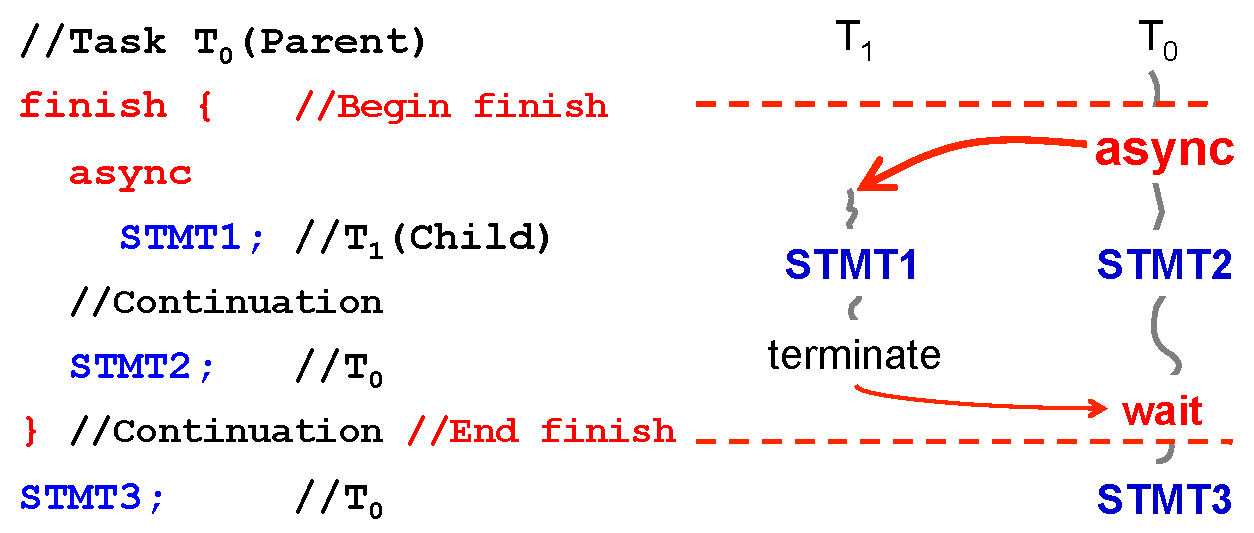
\includegraphics[width=3.25in]{../figs/async-finish}
\caption{An example with {\tt async} and {\tt finish}.}
\label{fig:async-finish}
\end{figure}


\section{Habanero Programming Model}

The Habanero programming model is built around a task-parallel view of
concurrency \cite{Cave:2011:HNA:2093157.2093165}. \figref{fig:async-finish} illustrates Habanero in its
simplest form \cite{Cave:2011:HNA:2093157.2093165}.

The \texttt{async}-construct is a mechanism for
creating a new asynchronous task: {\tt async}
$\langle${\em stmt}$\rangle$ causes the calling task (i.e., the
parent) to create a new child task to execute {\em
  $\langle$stmt$\rangle$} (logically) in parallel with the parent
task. {\em $\langle$stmt$\rangle$} can read or write any data in the
heap and can read (but not write) any local variable belonging to the
parent task's lexical scope. The task created by any
\texttt{async}-construct is scheduled at the point it is declared in
the program.

The \texttt{finish}-construct is a generalized join operation for
collective synchronization: {\tt finish} $\langle${\em
  stmt}$\rangle$ causes the parent task to execute {\em
  $\langle$stmt$\rangle$} and then wait until all tasks created within
{\em $\langle$stmt$\rangle$} have completed, including transitively
created tasks.  Each dynamic instance of a task has a unique {\em
  immediately-enclosing-finish} (IEF) during program execution. That IEF is the
innermost {\tt finish}-construct containing the task.  There is an implicit {\tt
  finish}-construct surrounding the entry point of the program so the program only terminates after
all tasks have completed.

A computation graph illustrating the semantics of the \texttt{async}
and \texttt{finish} constructs is on the right side of
\figref{fig:async-finish}. In the graph, task $T_0$ enters the
\texttt{finish}-construct, creates task $T_1$ at the
\texttt{async}-construct, and then continues on to
\texttt{STMT2}. After \texttt{STMT2}, $T_0$ waits for $T_1$ to
complete before moving on to \texttt{STMT3}. Note that \texttt{STMT1}
and \texttt{STMT2} are not ordered by the semantics and represent
parallel execution.

Habanero supports more advanced forms of tasking beyond creation and
collective synchronization. The \texttt{isolated}-construct, {\tt isolated}~$\langle${\it
  stmt1}$\rangle$, ensures that $\langle${\it stmt1}$\rangle$ is
evaluated in mutual exclusion with all other {\tt
  isolated}-constructs.  There are two subtle nuances in the Habanero
model for the \texttt{isolated}-construct:
\begin{compactenum}
\item The construct ensures mutual exclusion between \texttt{isolated}-constructs and not mutual exclusion on a particular memory location. Mutual exclusion on a particular memory location is implemented by wrapping operations on that memory location in \texttt{isolated}-constructs. 
\item Any Habanero implementation may relax mutual-exclusion between
  \texttt{isolated}-constructs as long as the constructs do not
  interfere with one another. Interference in this context means that
  multiple \texttt{isolated}-constructs access a common memory
  location and at least one of those accesses is a write.
\end{compactenum}

The \texttt{future}-construct lets tasks
return values to other tasks: \textbf{future} {\em f} $=$ \textbf{async}
  $\langle${\em expr}$\rangle$ creates a new child task to evaluate $\langle${\em expr}$\rangle$.  The local
variable {\em f} contains a \emph{future handle} to the newly created
task that can be used to obtain the value produced by $\langle${\em expr}$\rangle$. The blocking operation {\em f.get()} returns that value when the
child task completes.

The most complex construct in the Habanero model is the
\textit{phaser} \cite{Shirako:2008:PUD:1375527.1375568}. A phaser is a form of a barrier that provides
point-to-point fine-grain synchronization between tasks to coordinate
their movement through \emph{phases} of computation. Like barriers, phasers order execution of
portions of the program into phases and restrict tasks from
entering the next phase until the current phase is complete. Unlike
barriers though, phasers allow tasks to specify point-to-point relationships on
multiple phasers, and tasks can dynamically join or leave the phaser.

Tasks register with an instance of a phaser, and on registration,
declare the mode that control how that task
synchronizes relative to other tasks registered on the same
barrier. Synchronization takes place with the \texttt{next}-construct
which may block depending on the state of the phaser, and on how the task is registered with the phaser.
\begin{compactitem}
\item \texttt{SIG}: signal registration means all tasks that have designated themselves as signalers must signal the phaser
in order for the phase to advance.  The \texttt{next}-construct for a signal-only task signals the phaser and immediately advances to the next phase.  The phaser remembers each phase completed by any task.
\item \texttt{SIG\_WAIT}: \emph{signal-wait} registration means the task signals the phaser and then waits for other tasks to complete the phase. This registration mode functions like a traditional barrier. The \texttt{next}-construct for a signal-wait task reports phase completion and then blocks for the other signalers to complete the phase too.
\item \texttt{WAIT}: \emph{wait} registration means that the task blocks at the \texttt{next}-construct until the phase advances. 
\end{compactitem}
Phasers may also be bounded to specify slack in the number of phases that may separate
waiters and signalers so signalers can work ahead of waiters
up to a bound.\footnote{Omitted in this presentation of phasers is the ability of a single task to execute constructs after the end of one phase and before the start of the next phase.}

Habanero includes several other constructs such as
\texttt{foreach}-constructs, \texttt{forall}-constructs, \emph{data
  driven futures}, \emph{actors}, etc. most of which are syntactic
sugar for the presented constructs.


\section{Permission Regions}

\begin{figure}[t]
  \centering
  \scalebox{0.4}{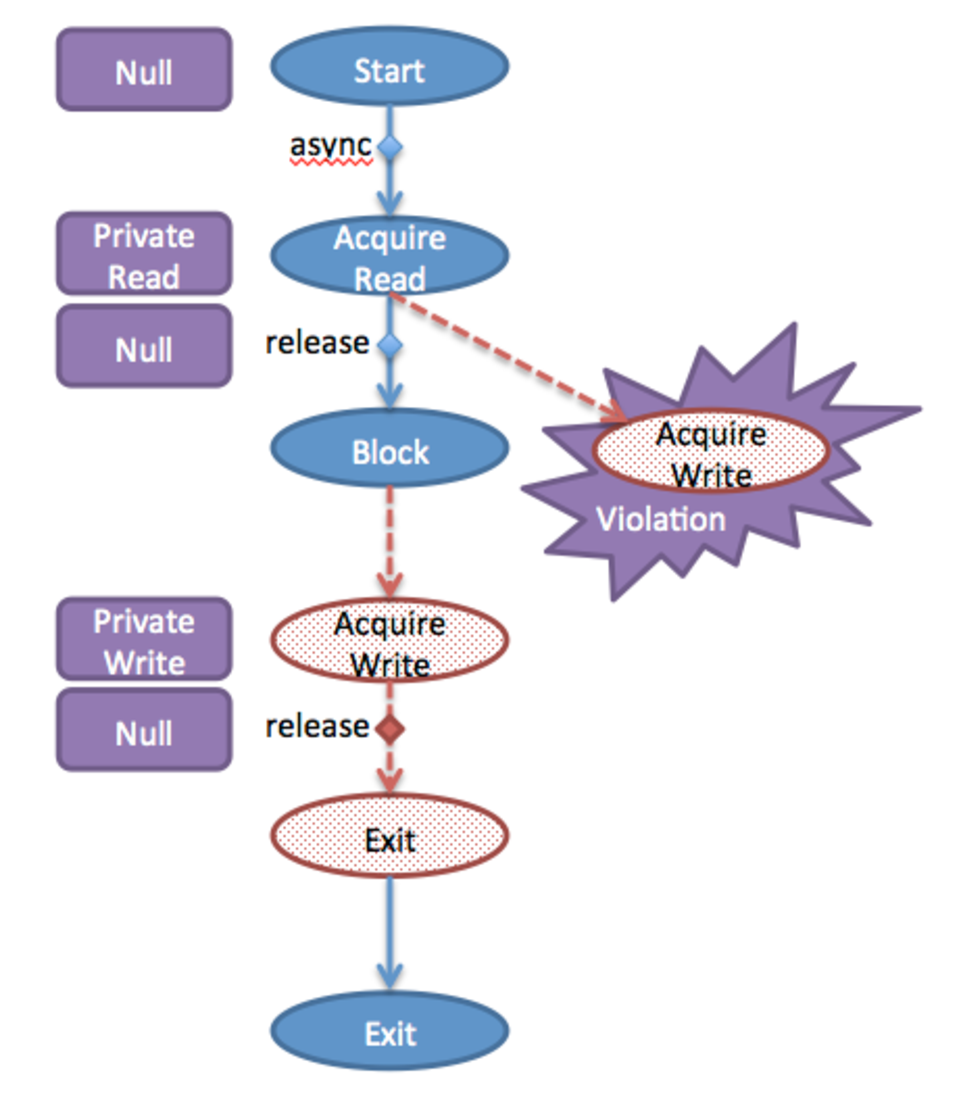
\includegraphics{../figs/stack-violation}}
  \caption{Different schedules for a permission region annotated
    version of the program in \figref{fig:hj-async-finish} with the
    schedule in the right branch reporting a permission violation.}
  \label{fig:permission-violation-state}
\end{figure}

Permission regions are programmer added annotations on shared objects
\cite{Westbrook:2011:PRR:2341616.2341627,Westbrook:2012:PPR:2367163.2367201}. The regions are indicated
as accessing shared objects in read or write mode. When the program
executes with run-time checking of permission regions enabled, a state machine is associated with each shared object to track
permissions on that object as indicated by the program annotations. If
accesses from distinct tasks on the same object conflict (i.e., a read
with a write or a write with a write), then a permission violation, indicative of a data race, is detected. An absence of violations implies an absence of any data races. 

To annotate the program in \figref{fig:hj-async-finish} with
permission regions, \lineref{line:push} and \lineref{line:peek} are
wrapped in separate regions, writing and reading, respectively, as follows:
\begin{lstlisting}
acquireW(stk);
stk.push(5);
releaseW(stk);
\end{lstlisting}
\begin{lstlisting}
acquireR(stk);
stk.peek();
releaseR(stk);
\end{lstlisting}
%Permission regions are transitive and span all the code in the
%\texttt{stk.push} and \texttt{stk.peek} methods.

The state machine associated with each region to track accesses and
detect violations is not shown due to space limitations, but it is intuitively
understood from the two possible task schedules in
\figref{fig:permission-violation-state} for an annotated version of the
program in \figref{fig:hj-async-finish}. The solid filled ovals and
solid lines represent the parent task and the dotted filled ovals and
dashed lines represent the child task created by the
\texttt{async}-statement on \lineref{line:async}. The squares indicate the current state of
the state machine that is tracking accesses to the shared object
\texttt{stk}.

The left branch of the tree is the schedule where the parent task runs
until it is blocked to wait for the child task. The parent task acquires
and releases private read privileges on the region and then the newly
created task runs, acquiring and releasing private write
privileges. If this schedule is followed in the run-time, then the
permission violation in the program is undetected. The right branch is another
possible schedule in the run-time. Here the child task runs just after
the parent task acquires private read privileges on {\tt stk}. When the
child task tries to acquire write privileges on {\tt stk}, its
state machine detects the violation.

Permission regions are distinctly different from mutual exclusion primitives such as locks and the Habanero 
\texttt{isolated}-construct. The \texttt{isolated}-construct defines
an atomic region that runs mutually exclusive to any other
\texttt{isolated}-construct and can be used to express  non-determination that is
intended by the programmer.  As such, isolated atomic regions are
serialized with respect to one another. Permission regions do not
include any serialization or synchronization semantics by themselves; rather, they check if concurrent accesses obey the permission annotations.

\section{JPF and VR}

JPF and VR both use Java reflection. When the user verifies an HJ program, the user runs JPF with VR as the target, and the HJ program as the input to the target. JPF uses reflection to open VR with the HJ program as an argument. VR in turn uses reflection to create a new thread to execute the HJ program and gives any remaining arguments as arguments to the HJ program. Reflection is intentional because VR has to be flexible to run an HJ program specified by the user and still provide functionality to HJ semantics. However, any property violations that JPF finds are within the HJ program and not within VR or JPF.

\begin{comment}
\begin{figure}
\begin{center}
{\small
\begin{verbatim}
public static void main (String args[]) {
   Class<?> verifyClass = 
      Class.forName((args[0])+"$Main");
   Class<?> stringArrayClass = args.getClass();
   Constructor<?> constructor = 
      verifyClass.getConstructor(stringArrayClass);
   String[] newArgs = new String[args.length -1];
   for (int i = 0; i < args.length-1; i++)
      newArgs[i] = args[i+1];
   java.lang.Object object = 
      constructor.newInstance(
         (java.lang.Object) newArgs);
   Class<?> thread = Class.forName("java.lang.Thread");
   Method method = thread.getDeclaredMethod("start");
   method.invoke(object, (java.lang.Object[]) null);}
\end{verbatim}
}
\end{center}
\caption{A simplified version of the main method in VR.}
\label{fig:main}
\end{figure}
\end{comment}

VR heavily relies on the soundness of JPF, and JPF's race detector. JPF's soundness is based on its partial order reduction and global search object ID. JPF's partial order reduction is critical: JPF must produce and examine essential interleaves for each thread and stop at locations where a data race occurs for checking. JPF does this by creating \texttt{ChoiceGenerators}, copying the current state of the machine, at certain parts of thread execution. JPF then systematically explores the state space, executing one thread at a time, which is called state expansion. The global search object ID is necessary for checks to ensure objects used by two threads are the same, even at different choice generators. JPF's \texttt{PreciseRaceDetector} from the default distribution is important because it checks for and reports data races that JPF has located.

VR was made with the intention to be used for verification, specifically by JPF. It was built in the simplest way possible to still produce correct results. We did not include any specific optimizations. To increase efficiency, an optimized scheduler can be integrated that is more suited with VR for scheduling, state expansion, and executing different interleavings than the default JPF scheduler factory.

The default JPF scheduler factory produces choice generators at several key locations in the partial order reduction, such as thread creation, thread termination, shared field access, monitor access, etc. However, not all state expansions from choice generators are interesting or relevant to VR. The optimized scheduler will only create choice generators for thread creation, shared array element access, and shared field access. \figref{fig:pseudocode} shows  psuedocode for the optimized scheduler. The optimized scheduler thus creates a smaller state space for JPF to verify than the default scheduler and removes the unnecessary choice generators that the default scheduler gives: thread suspense, thread resume, thread sleep, thread interrupt, thread yield, thread notify, thread terminate, shared object expose, wait, monitor enter, monitor exit, sync method enter, and sync method exit. Even after removing all these choice generators, the optimized scheduler still offers the same data race freedom guarentees that the default scheduler does. The optimized scheduler is given in the same repository as VR.

\begin{figure}
\begin{center}
{\small
\begin{verbatim}
createCG (string type, Thread[] threadsAvailable) {
    if (type.equals("THREAD_START"))
      createDefaultCG(type,threadsAvailable);
    else if (type.equals("SHARED_ARRAY_ACCESS"))
        createDefaultCG(type,threadsAvailable);
    else if (type.equals("SHARED_FIELD_ACCESS"))
        createDefaultCG(type,threadsAvailable);
    else
        noChoiceGenerator();}
\end{verbatim}
}
\end{center}
\caption{Psuedocode for the optimized scheduler.}
\label{fig:pseudocode}
\end{figure}
\section{Discussion}
\label{sec:discussion}

\subsection{Comparison to other languages}

Our analysis operates on a language that is similar to Habanero Java,
which is itself based on X10. Unlike our language, Habanero Java
distinguishes between futures and asynchronous procedures. The effect
is that every wait on a region waits for everything in that region. On
the other hand, Habanero Java allows asynchronous procedures' return
value handlers to have side effects, which can create data races.

Cilk has the same ability to post asynchronous threads and wait on all
of them to terminate with the same nondeterminism in the order that
threads join. In Cilk, return value handlers are called inlets and can
combine with nondeterministic thread joining order to create data
races. Cilk++ and Cilk Plus lack inlets.

Multilisp also includes futures. Its pcall mechanism is equivalent to
posting the evaluation of each argument and then waiting for them to
all return.

It is possible to identify data races in side-effecting return value
handlers by enumerating all possible orderings. However, the number of
orderings is the factorial of the number of return value handlers.

One alternative approach to this problem is the replacement that
Cilk++ and Cilk Plus use; instead of allowing return value handlers at
all, they use associative operations to combine results from their
child tasks. Enforcing such a restriction on return value handlers
instead of eliminating them entirely allows programmers to handle
most tasks naturally with similarly strong results.

Reactive systems, such as ReactJS, keep a collection of tasks to
execute. At the end of the main function, the eventloop keyword is
reached and parallel tasks execute atomically in a nondeterministic
order. Each task may post additional tasks to the work queue. Our
language could model reactive systems directly with a nondeterministic
\post\ statement. Because of the structured nature of the parallelism
in such languages, it is possible to create a computation graph with
the main function preceding each task and with each task running
without order with respect to its peers. Tasks that generate others
(parents) must execute before their children do. However, many
reactive systems are designed to run indefinitely rather than to
terminate, which complicates the application of the computation graph
model.

\subsection{Side effects in return value handlers}
\label{sec:side-effects-rvhs}

Return value handlers execute in the context of the waiting thread.
When a thread waits on a region with multiple tasks, the order in
which they join is nondeterministic. This creates a situation where
nondeterminism occurs within a single thread. As such, it is possible
to introduce data races on thread-local variables if the return value
handlers can create side effects.

Naturally, it is possible to expand the definitions of \rv\ and \wv\
so that they consider all variables and not just shared variables. In
order to distinguish between identically-named variables in different
tasks, \rv\ and \wv\ would need to take the task ID into account. This
extension would make the language and analysis more general but could
make the analysis much slower.




\section{Implementation and Results}
\label{sec:res}

The data race detection technique described in this paper has been implemented for Habanero Java. It uses the verification runtime specifically designed to test HJ programs \cite{anderson2014jpf}. This runtime makes use of JPF to schedule and run the programs. JPF is essentially a fully customizable Java virtual machine. JPF is modified by removing its default scheduling-factory that inserts choices on all thread actions and accesses to shared variables. Instead, a new scheduling factory based on Algorithm \ref{algo:isolated} is employed for scheduling. The computation graphs are stored in a directed acyclic graph \cite{jgrapht}. The computation graphs are exported in the dot file format for convenience and as a way to understand the structure of the program \cite{graphviz}.

The data-race detector is created by implementing the methods in the \textit{PropertyListenerAdapter} to create the computation graph. When the runtime passes an object of the type \textit{Task} to the \texttt{objectCreated} method, the \textsc{Post} rule is invoked that adds a new node to the computation graph. When the \textit{stop-finish} is executed, the \textsc{Await-next} rule is invoked that creates a node in the graph to synchronize the tasks in the finish block. The \texttt{executeInstruction} method is used to track memory locations that are accessed by various tasks by updating the node with the location accessed by the task during the execution of that instruction.

The results for this technique have been compared to two approaches implemented by JPF: \textit{Precise race detector} and \textit{Gradual permission regions} on benchmarks that cover a wide range of functionality in HJ. These two approaches are specifically chosen for comparison since the results generated by these approaches are sound for a given input just like the technique discussed in this paper. The results show a significant improvement in the time required for verification. 

The benchmarks used in this study make use of various HJ constructs for achieving task parallelism. They spawn a wide range of tasks with smaller programs having 3-15 tasks going all the way up to 525 tasks for larger programs. The experiments were run on a machine with an Intel Core i5 processor with 2.6GHz speed and 8GB of RAM.

\begin{table*}
\centering
\caption{Benchmarks of HJ programs: Computation graphs vs Permission Regions vs. PreciseRaceDetector}
\rowcolors{1}{light-gray}{white}
\label{tab:results}
\resizebox{\textwidth}{!}{
\begin{tabular}{|m{3.5cm}|c|c|c|c|c|c|c|c|c|c|c|}
\hiderowcolors
\hline
        &      &       & 
        \multicolumn{3}{c|}{\textbf{\textit{Computation graphs}}} & 
		 \multicolumn{3}{c|}{\textbf{\textit{Gradual permission regions}}} &
		\multicolumn{3}{c|}{\textbf{\textit{Precise race detector}}} \\ \hline
		
\textbf{Test ID }& \textbf{SLOC} & \textbf{Tasks} 
& \textbf{States}  & \textbf{Time}  & \textbf{Error Note }
& \textbf{States}  & \textbf{Time}  & \textbf{Error Note }
& \textbf{States}  & \textbf{Time}  & \textbf{Error Note }     \\ \hline

\showrowcolors

\textit{Primitive Array Race} & 39 & 3 
%& 5 & 00:00 & Race
& 5 & 00:00 & Race
& 5 & 00:00 & Race
& 220 & 00:00 & Race \\ \hline

\textit{Substring Search}  & 83 & 59 
%& 64 & 00:03 & Race
& 64 & 00:03 & Race
& 8 & 00:00 & Race 
& N/A & N/A & N/A \\ \hline

\textit{Reciprocal Array Sum} & 58 & 2
%& 12 & 0:00:16 & Race
& 4 & 00:08 & Race
& 32 & 00:06 & Race
& N/A & N/A & N/A \\ \hline

\textit{Primitive Array No Race} & 29 & 3 
%& 5 & 00:00 & No Race
& 5 & 00:00 & No Race
& 5 & 00:00 & No Race 
& 11,852 & 00:00 & No Race \\ \hline

\textit{Two Dim Arrays }& 30 & 11 
%& 15 & 00:01 & No Race
& 15 & 00:00 & No Race
& 15 & 00:00 & No Race 
& 597 & 00:00 & Race* \\ \hline

\textit{ForAll With Iterable} & 38 & 2
%& 9 & 00:00 & No Race
& 9 & 00:00 & No Race
& 9 & 00:00 & No Race 
& N/A & N/A & N/A \\ \hline

\textit{Integer Counter  Isolated} & 54 & 10
%& 24 & 00:01 & No Race
& 24 & 00:01 & No Race
& 1,013,102 & 05:53 & No Race 
& N/A & N/A & N/A \\ \hline

\textit{Pipeline With Futures} & 69 & 5
%& 34 & 0:00:00 & No Race
& 34 & 00:00 & No Race
& 34 & 00:00 & No Race 
& N/A & N/A & N/A \\ \hline

\textit{Binary Trees }& 80 & 525 
%& 632 & 0:00:05 & No Race
& 630 & 00:25 & No Race
& 632 & 00:03 & No Race 
& N/A & N/A & N/A \\ \hline

\textit{Prime Num Counter} & 51 & 25
%& 776 & 00:01 & No Race
& 776 & 00:01 & No Race
& 3,542,569 & 17:37 & No Race 
& N/A & N/A & N/A \\ \hline

\textit{Prime Num  Counter ForAll}  & 52 & 25
%& 30 & 0:00:02 & Race*
& 30 & 00:02 & No Race
& 18 & 00:01 & No Race
& N/A & N/A & N/A \\ \hline

\textit{Prime Num Counter ForAsync}  & 44 & 11 
%& 653 & 0:00:01 & No Race
& 653 & 00:01 & No Race
& 2,528,064 & 15:44 & No Race 
& N/A & N/A & N/A \\ \hline

\textit{Add}  & 67 & 3 
%& 11 & 0:00:01 & No Race 
& 11 & 00:01 & No Race 
& 62,374 & 00:33 & No Race
& 4930 & 00:03 & Race* \\ \hline

\textit{Scalar Multiply}  & 55 & 3 
%& 15 & 0:00:01 & No Race
& 15 & 00:01 & No Race
& 55,712 & 00:30 & No Race 
& 826 & 00:01 & Race* \\ \hline

\textit{Vector Add} & 50 & 3 
%& 5 & 0:00:01 & No Race
& 5 & 00:00 & No Race
& 17 & 00:00 & No Race 
& 46,394 & 00:19 & No Race \\ \hline

\textit{Clumped Access}  & 30 & 3 
%& 9 & 0:00:07 & No Race
& 5 & 00:03 & No Race
& 15 & 00:00 & No Race 
& N/A & N/A & N/A \\ \hline

\end{tabular}}
\vspace{-1em}
\end{table*}

\tableref{tab:results} presents the results of verification of the HJ benchmarks. The number of states explored by JPF and time required for verification by each method is compared. The tests are run for a maximum of an hour before they are terminated manually. If a test does not finish in the time bound or if it runs out of JVM memory, then it is marked as N/A in the table. The error note column shows the results of verification. The tests that produce erroneous results are marked with an asterisk ($\ast$). 

The \textit{Precise race detector} explores all potential executions of the program in a systematic way. Each execution is a sequence of transitions. Each transition takes the system from one state to another. Each transition consists of a sequence of byte-code instructions. JPF groups byte-code instructions such that an instruction that manipulates a shared variable is the first one of a transition. In every state that JPF visits, the \textit{precise race detector} checks all actions that can be performed next. If this collection of actions contains at least two conflicting accesses to a shared variable, then a data-race on the shared variable is reported. The \textit{precise race detector} inserts choices in the scheduler for all thread actions such as thread creation, synchronizations, locks etc. Therefore, it does not complete execution within the stipulated time or runs out of memory even on smaller programs because of the state space explosion. It also reports race for \textit{Two Dimensional Arrays}, \textit{Scalar multiply} and \textit{Vector Add} benchmarks where no data race actually exists in the program. This error is because in precise race detector, the access on an array object looks like a data race since it is not able to see the difference in the indexes.

\textit{Gradual permission regions} use program annotations to reduce the state space of the program \cite{mercer2015model}. Whenever a shared variable is accessed by multiple tasks in the program, the accesses have to be annotated to inform the data-race detector to create different schedules for these accesses. It is prone to human errors because of the need for manual annotation. If the program is annotated incorrectly, the results of data race detection analysis are no longer sound. \textit{gradual permission regions} works better than \textit{precise race detector}. Compared to \textit{computation graphs} in this paper though it falls behind quickly when there are several regions to annotate. A single execution is all that is needed for the \textit{computation graph analysis} while \textit{permission regions} have to enumerate an exponential number of schedules over the regions. The difference in performance is seen in the \textit{Add}, \textit{Scalar multiply} and \textit{Prime number counter} benchmarks. These benchmarks use shared variables that have to be enclosed within regions which results in a large state space for permission regions. The \textit{Prime number counter} benchmark also has isolated sections and therefore, the state space for \textit{computation graphs} is also large compared to other benchmarks.

We also evaluated our data race detector on some real world benchmarks. The \textit{Crypt-af} and \textit{Crypt-f} benchmarks are implementation of the IDEA encrytion algorithm and \textit{Series-af} and \textit{Series-f} are the Fourier coefficient analysis benchmarks adapted from the JGF suite \cite{bull2000benchmark} using \textbf{async-finish} and \textbf{future} constructs respectively. The \textit{strassen} benchmark is adapted from the  OpenMP version of the program in the Kastors suite \cite{virouleau:hal-01081974}. \tableref{tab:results1} shows the results of this evaluation.

\begin{table*}
\centering
\caption{Evaluation of Computation graphs on real world benchmarks}
\rowcolors{1}{light-gray}{white}
\label{tab:results1}
\begin{tabular}{|c|c|c|c|c|c|}
\hiderowcolors
\hline

\textbf{Test ID }& \textbf{SLOC} & \textbf{Tasks} 
& \textbf{States}  & \textbf{Time}  & \textbf{Error Note }\\ \hline

\showrowcolors

\textit{Crypt-af} & 1010 & 259
& 260 & 00:17 & No Race  \\ \hline

\textit{Crypt-f}  & 1145 & 387 
& 775 & 00:46 & No Race \\ \hline

\textit{Series-af} & 730 & 329
& 750 & 00:36 & No Race \\ \hline

\textit{Series-f} & 830 & 354 
& 630 & 00:51 & No Race\\ \hline

\textit{Strassen} & 560 & 3
& 7 & 00:57 & No Race \\ \hline

\end{tabular}
\vspace{-1em}
\end{table*}
\vspace{-2em}
\section{Conclusion} \label{sec:conclusion}
This work presents a sound and complete technique for data race detection in task parallel programs using computation graphs.  The computation graph creation is presented with the formal semantics for task parallel languages. A scheduling algorithm to create all computation graph structures for programs containing mutual exclusion is also presented for use in model checking. The data race detection analysis is implemented for a Java implementation of the Habanero programming model using JPF and evaluated on a host of benchmarks. The results are compared to JPF's precise race detector and a gradual permission regions based extension. The results show that computation graph analysis reduces the time required for verification significantly relative to JPF's standards. 

\begin{comment}
This work can be extended in the following ways:
\begin{itemize}
\item The data race detector based on computation graphs explores just one control flow path that is taken by the program execution based on the input. The listener can be extended to explore other control flow paths by using Symbolic Execution.
\item The computation graphs can be created statically using program instrumentation and analyzed to gain performance improvements.
\end{itemize}
\end{comment}

\bibliographystyle{abbrv}
\bibliography{../bib/paper}  
\balancecolumns
\end{document}
